\documentclass{article}
\usepackage{amsmath}
\usepackage[utf8]{vietnam}
\usepackage{braket}
\usepackage[a4paper,tmargin=2.0cm, bmargin=2.5cm,lmargin=2.5cm, rmargin=2.5cm]{geometry}
\usepackage{array}
\usepackage{amsthm, amssymb, mathtools, mathrsfs, systeme, amsmath}
\usepackage{graphicx, wrapfig} %chèn hình
\usepackage{booktabs}
\usepackage{multicol, parcolumns}
\usepackage{fancyhdr,LastPage}
\pagestyle{fancy}
\title{Quantum Optics - tuần 2}
\author{Nguyễn Minh Hiền}
\date{\today}
\lhead{Ho Chi Minh University of Science}
\rfoot{First exercise}
\cfoot{Page \thepage\ / \pageref{LastPage}}
\begin{document}
	\maketitle
\section*{Quy tắc chọn lọc lưỡng cực điện}
Phần tử ma trận lưỡng cực điện được cho trong phương trình 4.18 có thể dễ dàng đánh giá cho các nguyên tử đơn giản với các hàm sóng đã biết. Điều này dẫn đến khái niệm về quy tắc chọn lọc (có khi gọi là quy tắc lọc lựa) lưỡng cực điện. Đây là các quy tắc về các số lượng tử của các trạng thái ban đầu và trạng thái cuối. Nếu các trạng thái không thỏa mãn quy tắc chọn lọc, thì tốc độ chuyển tiếp lưỡng cực điện sẽ bằng không.\\

Các chuyển tiếp tuân theo quy tắc chọn lọc lưỡng cực điện được gọi là chuyển tiếp được phép, trong khi những chuyển tiếp không tuân theo được gọi là chuyển tiếp bị cấm. Các chuyển tiếp được phép E1 có xác suất chuyển tiếp cao và do đó có thời gian sống bức xạ ngắn, thường nằm trong khoảng từ 1–100 ns (xem Bảng 4.1).\\ Ngược lại, các chuyển tiếp bị cấm chậm hơn nhiều. Các thang thời gian khác nhau giữa chuyển tiếp được phép và bị cấm dẫn đến một sự phân loại khác của quá trình phát xạ tự phát, được gọi là huỳnh quang và lân quang, tương ứng. Huỳnh quang là quá trình "nhanh" trong đó photon được phát ra trong vòng vài nanosecond sau khi nguyên tử bị kích thích, trong khi lân quang là quá trình phát xạ "chậm" kéo dài một thời gian đáng kể.\\

Quy tắc chọn lọc lưỡng cực điện cho một electron đơn trong hệ hydro với các số lượng tử l, m, s và ms được tóm tắt trong Bảng 4.2.\\
\begin{center}
\begin{tabular}{|c|c|c|}
	\hline
	Quantum number & Selection rule & Polarization \\
	\hline
	Parity & Changes & \\
	\hline
	$l$ & $\Delta l = \pm 1$ & \\
	\hline
	$m$ & $\Delta m = +1$ & Circular: $\sigma^{+}$ \\
	\cline{3-3}
	& $\Delta m = -1$ & Circular: $\sigma^{-}$ \\
	\cline{3-3}
	& $\Delta m = 0$ & Linear: $\parallel z$ \\
	\hline
	$s$ & $\Delta s = 0$ & \\
	\hline
	$m_s$ & $\Delta m_s = 0$ & \\
	\hline
\end{tabular}
\end{center}
 Nguồn gốc của các quy tắc này là như sau:
\begin{itemize}
	\item Quy tắc thay đổi đối xứng parity xuất phát từ thực tế rằng toán tử lưỡng cực điện tỷ lệ thuận với r, nên là một hàm lẻ.
	\item Quy tắc cho $\Delta l$ bắt nguồn từ các tính chất của các hàm cầu điều hòa và phù hợp với quy tắc đối xứng vì các hàm sóng có đối xứng parity là $(-1)^l$.
	\item Quy tắc cho $\Delta m$ có thể được hiểu bằng cách nhận ra rằng các photon phân cực tròn $\sigma^+$ và $\sigma^-$ mag moment động lượng $\hbar$ và $-\hbar$ dọc theo trục z, và do đó m phải thay đổi một đơn vị để bảo toàn mômen góc. Đối với ánh sáng phân cực thẳng dọc theo trục z, các photon không mang thành phần mômen theo trục z, dẫn đến $\Delta m = 0$ trong khi ánh sáng phân cực theo trục x hoặc y có thể được coi là sự kết hợp đồng thời của các photon $\sigma^+$ và $\sigma^-$ cho $\Delta m = \pm 1$.
	\item Quy tắc chọn lọc spin xuất phát từ thực tế là photon không tương tác với spin của electron, do đó các số lượng tử spin không bao giờ thay đổi trong quá trình chuyển tiếp.
\end{itemize}
Những quy tắc chọn lọc này có thể được tổng quát hóa lên cho nguyên tử đa electron (với các số lượng tử L,S,J) như sau:
\begin{itemize}
	\item Parity của hàm sóng phải thay đổi
	\item $\Delta L =\pm 1$ cho electron đổi trạng thái
	\item $\Delta L=0. \pm 1$ nhưng L chuyển từ 0 thành 0 thì bị cấm
	\item  $\Delta J=0. \pm 1$ nhưng J chuyển từ 0 thành 0 thì bị cấm
	\item $\Delta S = 0$
\end{itemize}
Quy tắc chọn chẵn lẻ xuất phát từ tính lẻ của toán tử lưỡng cực điện. Quy tắc về số lượng tử l áp dụng quy tắc một electron cho electron riêng lẻ thực hiện quá trình chuyển tiếp. Các quy tắc về L và J bắt nguồn từ thực tế là photon mang một đơn vị mômen động lượng. Quy tắc cuối cùng là hệ quả của việc photon không tương tác với spin.\\

Các quy tắc chọn cho các quá trình chuyển tiếp cấp cao hơn là khác nhau. Ví dụ, các quá trình chuyển tiếp lưỡng cực từ và tứ cực điện có thể xảy ra giữa các trạng thái có cùng tính chẵn lẻ.\\
Điều này cho phép một nguyên tử ở một trạng thái kích thích không thể phân rã bằng quá trình chuyển tiếp lưỡng cực điện để trở về trạng thái cơ bản. Trong các trường hợp cực đoan, có thể xảy ra tất cả các loại chuyển tiếp bức xạ photon đơn tiêu chuẩn đều bị cấm. Trong trường hợp này, trạng thái kích thích được gọi là metastable, và nguyên tử phải giải phóng năng lượng bằng cách truyền năng lượng của nó cho các nguyên tử khác trong các va chạm, hoặc bằng một số cơ chế có xác suất thấp khác mà chúng ta chưa xem xét ở đây, chẳng hạn như phát xạ đa photon.\\

Các trạng thái metastable đóng vai trò quan trọng trong nhiều lĩnh vực của vật lý và công nghệ. Ví dụ, chúng được sử dụng trong đồng hồ nguyên tử để tạo ra các tiêu chuẩn thời gian cực kỳ chính xác. Ngoài ra, các trạng thái metastable cũng được ứng dụng trong laser, quang học lượng tử và nghiên cứu về các quá trình cơ bản trong vật chất. Thời gian sống của một trạng thái metastable có thể rất khác nhau, từ vài nano giây đến hàng giờ hoặc thậm chí lâu hơn, tùy thuộc vào cấu trúc năng lượng của nguyên tử và các yếu tố môi trường xung quanh.
\section*{Bề rộng và dáng điệu của phổ}
Xét một "vạch phổ", như thường được quan sát trong các môn thực nghiệm. Những tưởng "vạch" ấy chỉ đơn giản là một vạch theo nghĩa toán học, tức chỉ một giá trị hoàn toàn xác định. Tuy nhiên, thực tế "vạch" ấy lại là một tập hợp nhiều giá trị xung quanh một giá trị nào đấy, tạo nên một "phân bố" có dạng hình chuông, gọi là hàm "spectral lineshape" $g_\omega(\omega)$.
Ta dễ thấy dạng hình "quốc dân" của phân bố Gauss:\\
\begin{center}
	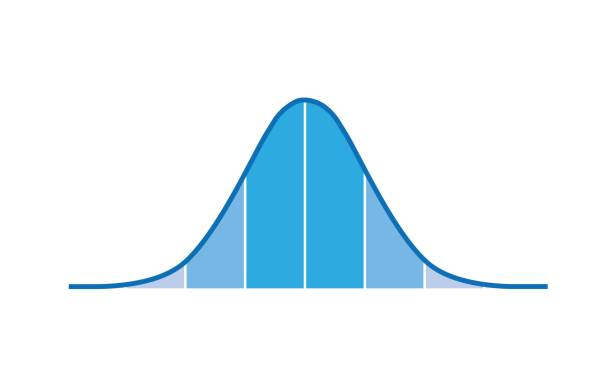
\includegraphics{gauss.jpg}\\
\end{center}
hoặc cũng có thể là Lorentz:
\begin{center}
	\includegraphics[scale=0.5]{cauchy.png}\\
\end{center}
Giá trị trung tâm được xác định bởi $$\hbar\omega_0=E_2-E_1$$ và được chuẩn hóa: $$\int_{0}^{\infty}g_\omega(\omega)d\omega=1$$
Đại lượng quan trọng nhất cần được xác định là Full Width at Half Maximum (FWHM), tức độ rộng tại phân nửa độ cao cực đại, cho ta biết độ rộng của phổ.\\
Thường có ba nguyên nhân ảnh hưởng đến độ rộng phổ:
\begin{itemize}
	\item thời gian sống (lifetime (natural) broadening)
	\item va chạm (collisional (pressure) broadening)
	\item Doppler
\end{itemize}
\subsection*{Lifetime broadening}
Ta đã biết liên hệ giữa hệ số Einstein A và thời gian sống $\tau$. Thời gian sống này liên hệ với năng lượng bức xạ (tức sự mở rộng của phổ) qua Bất định Heisenberg $$\Delta E\Delta t\gtrsim \hbar$$
and $$\Delta E = \hbar\Delta\omega$$
so $$\Delta \omega=\frac{\Delta E}{\hbar}\gtrsim\frac{1}{\tau}$$
Ta có hàm mô tả dạng phổ $$g(\omega) = \frac{\Delta\omega}{2\pi} \frac{1}{(\omega - \omega_0)^2 + (\Delta\omega/2)^2}$$
và dáng hình của nó:
\begin{center}
	\includegraphics[scale=0.75]{g(w).png}\\
\end{center}
\subsection*{Collisional broadening}
Các phân tử có thể va đập, với nhau và với thành bình, khiến thời gian "sống" bị giảm đi (năng lượng bị mất nhanh hơn).\\
Bằng thống kê, ta có: $$\tau_{\text{collision}} \sim \frac{1}{\sigma_s P} \left( \frac{\pi m k_B T}{8} \right)^{1/2}$$ với $\sigma_s$ là tiết diện va chạm và P là áp suất. Khi ấy, collisional broadening còn được gọi là pressure broadening.\\
Trong trường hợp này, thời gian sống thường là rất ngắn, dẫn đến độ rộng phổ thật lớn so với trường hợp "natural".\\
Vậy nên ta có thể khắc phục bằng cách giảm thiểu áp suất P, đó là lí do ta sử dụng các đèn áp suất thấp trong khảo sát phổ.\\
\begin{center}
	\includegraphics[scale=0.75]{pbroad.png}\\
\end{center}
\subsection*{Doppler broadening}
Việc các hạt nguyên tử di chuyển lại gần hay ra xa khỏi máy đo cũng ảnh hưởng đến phổ, khi ta xét hiệu ứng Doppler là đáng kể. \\
Khi hạt di chuyển lại gần máy đo, ta có $$\omega=\omega_0\left(1+\frac{v_x}{c}\right)$$
Số hạt di chuyển với vận tốc $v_x$ đến $v_x+dv_x$ được cho bởi cơ học thống kê: $$N(v_x) = N_0 \left( \frac{2k_B T}{\pi m} \right)^{1/2} \exp \left( -\frac{m v_x^2}{2k_B T} \right)$$ với FWHM được cho bởi $$\Delta \omega_{\text{Doppler}} = 2 \omega_0 \left( \frac{(2 \ln 2) k_B T}{mc^2} \right)^{1/2} = \frac{4 \pi}{\lambda} \left( \frac{(2 \ln 2) k_B T}{m} \right)^{1/2}$$
\section*{LASER}
Từ "laser" là từ viết tắt của cụm từ "Light Amplification by Stimulated Emission of Radiation" (khuếch đại ánh sáng bằng phát xạ kích thích). Laser hoạt động lần đầu tiên được chứng minh vào năm 1960, và từ đó, laser đã trở thành công cụ thiết yếu trong quang học phi tuyến và lượng tử. Trong phần này, chúng ta sẽ đưa ra một cái nhìn tổng quan ngắn gọn về các nguyên lý vật lý cơ bản của hoạt động laser, và sau đó mô tả ngắn gọn các đặc tính chính của các loại laser thường được sử dụng trong phòng thí nghiệm.
\section*{FOX's exercises}
\subsection*{4.2}
\textit{Show that the parities of the initial and final states involved in E1 transitions must be different.}\\
Hơi ăn gian một xíu, ta viết trạng thái đầu và cuối dưới dạng quen thuộc hơn, lần lượt là $|n,l,m\rangle$ và $|n',m',l'\rangle$.\\
Xét toán tử dipole $$\textbf{p}=-e.\textbf{r}$$
Cho toán tử parity tác động lên:$$\hat{\pi}^\dagger \textbf{p}\hat{\pi}=-\textbf{p}$$
Ta đồng thời cũng có $$\hat{\pi}\psi(\theta,\phi)=(-1)^l\psi(\theta,\phi)$$\\
Khi đó, ta có xác suất chuyển dời:
\begin{equation}
	\begin{split}
		\bra{n',m',l'}\textbf{p}\ket{n,m,l}&=-\bra{n',m',l'}\hat{\pi}^\dagger \textbf{p}\hat{\pi}\ket{n,m,l}\\
		&=-(-1)^{l'}\bra{n',m',l'}\textbf{p}(-1)^l\ket{n,m,l}\\
		&=-(-1)^{l'+l}\bra{n',m',l'}\textbf{p}\ket{n,m,l}\\
	\implies 0&=\bra{n',m',l'}\textbf{p}\ket{n,m,l}\left(1+(-1)^{l'+l}\right)
	\end{split}
\end{equation}
Trường hợp hai trạng thái đầu và cuối trùng nhau, tức l = l', khi đó $$(-1)^{l'+l} = (-1)^{2l} = 1 \implies \left(1+(-1)^{l'+l}\right) =2 \neq 0 $$
buộc $$\bra{n',m',l'}\textbf{p}\ket{n,m,l} = 0$$
ứng với sự không chuyển dời, hay xác suất chuyển dời bằng không. Nên "the parities of the initial and final states involved in E1 transitions must be different".\\
\subsection*{4.3}
\subsubsection*{a) m'=m for $\hat{z}$-polarized light}
Xét hàm sóng của nguyên tử Hydrogen có dạng $$\psi(r, \theta, \phi) = F(r, \theta) \exp(im\phi)$$
Một cách ăn gian (lần nữa), ta có thể viết trạng thái của hàm sóng này dưới dạng $\ket{n,m,l}$. \\
Ta có các toán tử tác động lên:
\begin{itemize}
	\item $H\ket{n,m,l}$=$E_n\ket{n,m,l}$
	\item $L^2\ket{n,m,l}=\hbar^2l(l+1)\ket{n,m,l}$
	\item $L_z\ket{n,m,l}=m\hbar\ket{n,m,l}$
\end{itemize}
Giả sử V là một toán tử vector,  $V_\pm=V_x+iV_y$ (ứng với $\sigma^+$ và $\sigma^-$ trong Fox).
Ta có bộ giao hoán tử:
\begin{itemize}
	\item $[L_z,V_z]=0$
	\item $[L_\pm,V_\pm]=0$
	\item  $[L_\pm,V_z]=\mp \hbar V_\pm$
	\item $[L_\pm,V_\mp]=\pm2\hbar V_z$
\end{itemize}
Ta có:
\begin{equation}
	\begin{split}
		\bra{n',m',l'}[L_z,V_z]\ket{n,m,l}=0
	&\implies	\bra{n',m',l'}(L_z^\dagger V_z^\dagger-V_zL_z)\ket{n,m,l}=0\\
	&\implies (m'-m)\hbar\bra{n',m',l'}V_z\ket{n,m,l}=0\\
	\end{split}
\end{equation}
Để $\bra{n',m',l'}V_z\ket{n,m,l}\neq 0$, (m'-m) phải bằng 0. Như vậy, các phần tử ma trận bằng 0 trừ khi m'=m.\\
\subsubsection*{b) c) m'= m $\pm1$ for $\sigma^\pm$-polarized light}
Chứng minh tương tự, ta có
\begin{equation}
	\bra{n',m',l'}[L_z,V_\pm]\ket{n,m,l}=\pm\hbar<V_\pm>\\
	\implies (m'-m\mp 1)\hbar<V_\pm>=0\\
\end{equation}
Để $\bra{n',m',l'}V_\pm\ket{n,m,l}\neq 0$, (m'-m$\mp1$) phải bằng 0. Như vậy, các phần tử ma trận bằng 0 trừ khi m'=m$\pm1$.\\
\subsubsection*{d) m'=m$\pm1$ for $\hat{x}$ or $\hat{y}$-polarized light}
Ta có
\begin{equation}
	\begin{split}
	[L_z,x]&=[xp_y-yp_x,x]\\
	&=-y[p_x,x]\\
	&=-y(-i\hbar)\\
	&=iy\hbar
	\end{split}
\end{equation}
Chứng minh tương tự: $$[L_z,y]=-i\hbar x$$
Như vậy, ta có hệ phương trình:
\begin{itemize}
	\item (m'-m)$\hbar\bra{n',m',l'}x\ket{n,m,l}-i\hbar \bra{n',m',l'}y\ket{n,m,l}=0$
	\item $i\hbar \bra{n',m',l'}x\ket{n,m,l} + (m'-m)\hbar \bra{n',m',l'}y\ket{n,m,l}=0$
\end{itemize}
Ta thế phương trình trên xuống phương trình dưới, ta có:
$$i\hbar\frac{i\hbar\bra{n',m',l'}y\ket{n,m,l}}{\hbar(m'-m)}+(m'-m)\hbar \bra{n',m',l'}y\ket{n,m,l}=0\\
\Leftrightarrow \left[\frac{-\hbar}{m'-m}+\hbar(m'-m)\right]\bra{n',m',l'}y\ket{n,m,l}=0$$
để xác suất chuyển trạng thái khác 0, thì $\frac{-\hbar}{m'-m}+\hbar(m'-m)=0$
khi đó $$(m'-m)^2=1$$
Và như thế, mọi thành phần ma trận khác $(m'-m\pm1)$ thì bằng không.
\subsection*{4.4}
	To explain why the time-dependent electric field \(\mathcal{E}(t)\) is given in this form, consider the relationship between the intensity of light and the electric field.
	
	\subsection*{a) Intensity and Electric Field Relationship}
	
	The intensity \(I(t)\) of a wave is proportional to the square of the amplitude of the electric field:
	
	\[
	I(t) \propto |\mathcal{E}(t)|^2.
	\]
	
	Given that the intensity decays exponentially with time:
	
	\[
	I(t) = I(0) \exp(-t/\tau),
	\]
	
	we can infer that the electric field amplitude must also have an exponential decay factor to ensure that its square matches the intensity decay:
	
	\[
	|\mathcal{E}(t)|^2 = |\mathcal{E}_0|^2 \exp(-t/\tau).
	\]
	
	\subsubsection*{Form of the Electric Field}
	
	To satisfy the above relationship, the electric field \(\mathcal{E}(t)\) should include a time-dependent factor that decays as the square root of the intensity decay:
	
	\[
	\mathcal{E}(t) = \mathcal{E}_0 \exp(-t/2\tau).
	\]
	
	Additionally, the electric field of a wave with angular frequency \(\omega_0\) can be expressed as a cosine function:
	
	\[
	\mathcal{E}(t) = \mathcal{E}_0 \cos(\omega_0 t) \exp(-t/2\tau).
	\]
	
	This form satisfies the condition that the intensity \(I(t)\) will be proportional to the square of the electric field, resulting in an exponential decay with the same time constant \(\tau\).
	
	\subsubsection*{Explanation of the Conditions}
	
	- For \(t < 0\), \(\mathcal{E}(t) = 0\) because the burst of light has not yet been emitted.\\
	- For \(t \geq 0\), the electric field \(\mathcal{E}(t) = \mathcal{E}_0 \cos(\omega_0 t) \exp(-t/2\tau)\) models the oscillating nature of the light wave with an exponentially decaying amplitude, consistent with the given intensity profile.
To find the emission spectrum, we take the Fourier transform of the electric field \(\mathcal{E}(t)\).

\subsection*{b) Fourier Transform}

The electric field for \(t \geq 0\) is given by:

\[
\mathcal{E}(t) = \mathcal{E}_0 \cos(\omega_0 t) e^{-t/2\tau} = \frac{\mathcal{E}_0}{2} \left( e^{i\omega_0 t} + e^{-i\omega_0 t} \right) e^{-t/2\tau}.
\]

The Fourier transform \(\mathcal{E}(\omega)\) is:

\[
\mathcal{E}(\omega) = \frac{1}{\sqrt{2\pi}} \int_{-\infty}^{\infty} \mathcal{E}(t) e^{i\omega t} \, dt.
\]

Since \(\mathcal{E}(t) = 0\) for \(t < 0\), the integral becomes:

\[
\mathcal{E}(\omega) = \frac{1}{\sqrt{2\pi}} \int_{0}^{\infty} \left( \frac{\mathcal{E}_0}{2} e^{i(\omega_0 t - \omega t) - t/2\tau} + \frac{\mathcal{E}_0}{2} e^{-i(\omega_0 t + \omega t) - t/2\tau} \right) dt.
\]

\subsubsection*{Solving the Integrals}

Consider the first term:

\[
\int_{0}^{\infty} e^{i(\omega_0 - \omega)t - t/2\tau} \, dt = \int_{0}^{\infty} e^{-(1/2\tau - i(\omega_0 - \omega))t} \, dt.
\]

This evaluates to:

\[
\frac{1}{1/2\tau - i(\omega_0 - \omega)}.
\]

For the second term:

\[
\int_{0}^{\infty} e^{-i(\omega_0 + \omega)t - t/2\tau} \, dt = \frac{1}{1/2\tau + i(\omega_0 + \omega)}.
\]

\subsubsection*{Combining the Results}

\[
\mathcal{E}(\omega) = \frac{\mathcal{E}_0}{2\sqrt{2\pi}} \left( \frac{1}{1/2\tau - i(\omega_0 - \omega)} + \frac{1}{1/2\tau + i(\omega_0 + \omega)} \right).
\]

\subsubsection*{Assumption: \(\omega_0 \gg 1/\tau\)}

Given this assumption, the second term is negligible compared to the first, so:

\[
\mathcal{E}(\omega) \approx \frac{\mathcal{E}_0}{2\sqrt{2\pi}} \cdot \frac{1}{1/2\tau - i(\omega_0 - \omega)}.
\]

\subsubsection*{Emission Spectrum}

The intensity is proportional to the square of the Fourier transform magnitude:

\[
I(\omega) \propto |\mathcal{E}(\omega)|^2 = \left|\frac{\mathcal{E}_0}{2\sqrt{2\pi}} \cdot \frac{1}{1/2\tau - i(\omega_0 - \omega)}\right|^2.
\]

This results in a Lorentzian profile:

\[
I(\omega) \propto \frac{1}{(\omega - \omega_0)^2 + (1/2\tau)^2}.
\]

This matches the given expression for the emission spectrum.

\end{document}